\graphicspath{{literature_review/fig/}}

\chapter{Literature Review}
\section{Biosensors}
Biosensors are employed in applications such as disease monitoring, drug discovery, and detection of pollutants, disease-causing micro-organisms and markers that are indicators of a disease in bodily fluids (blood, urine, saliva, sweat).\cite{bhallaIntroductionBiosensors2016} 
\subsection{Background on Biomarkers}
A biomarker is an objective measure that that gives an indication of the biological processes happening inside the body at a given moment.\cite{BiomarkersNationalInstitute} They are physical substances found in the body that can be measured. The concentration of biomarkers differs between healthy individuals and individuals with diseases, thereby aiding in diagnosis and monitoring of diseases.\cite{rosenzweigWhatArePancreatic2018} Some biomarkers are easy to measure (such as blood pressure, body weight, etc.) while others require tests of blood, urine or tissue samples.\cite{BiomarkersNationalInstitute} 

This project will focus on the detection of biomarkers found in blood samples such as the CA-19 biomarker used for pancreatic cancer detection. \todo{Note: Verduidelik bietjie oor CA-19.} The concentration of these biomarkers in blood can give an indication of the presence and progression of a variety of diseases, including many types of cancer.\cite{ribeiroApplicationsElectrochemicalImpedance2024}

\subsection{Types of Biosensors}
A biosensor consists of an analyte, a bioreceptor and a transducer mechanism combined with the electronics needed to process the signal.\cite{bhallaIntroductionBiosensors2016} The analyte is the substance of interest (such as biomarkers) that needs detection. Bioreceptors are molecules such as enzymes, cells, DNA or antibodies that specifically recognise the analyte. These bioreceptors produce a signal (in the form of light, heat, pH, charge or mass change, etc.) when they interact with the analyte.\cite{bhallaIntroductionBiosensors2016} Antibody based biosensors are the type of biosensor that will be used to detect biomarkers in this project.

Antibodies are produced by vertebrates as part of their immune response to foreign organisms or substances (called antigens). They are the most common biorecognition element used in biosensors.\cite{zengRecombinantAntibodiesTheir2012} Antibodies are Y-shaped cells that can be divided into two distinct regions. The top of the Y is variable and binds to a specific antigen depending on the amino acids present in this region. The amino acids present in the constant region (the bottom of the Y) is similar between different classes of antibodies (within the same species of animal).\cite{zengRecombinantAntibodiesTheir2012} This constant region binds to the substrate of the biosensor during immobilization, leaving the variable region free to bind with antigens.\cite{suedaAntibodyImmobilizationImmunosensing2022a}
\begin{figure}[ht]
    \centering
    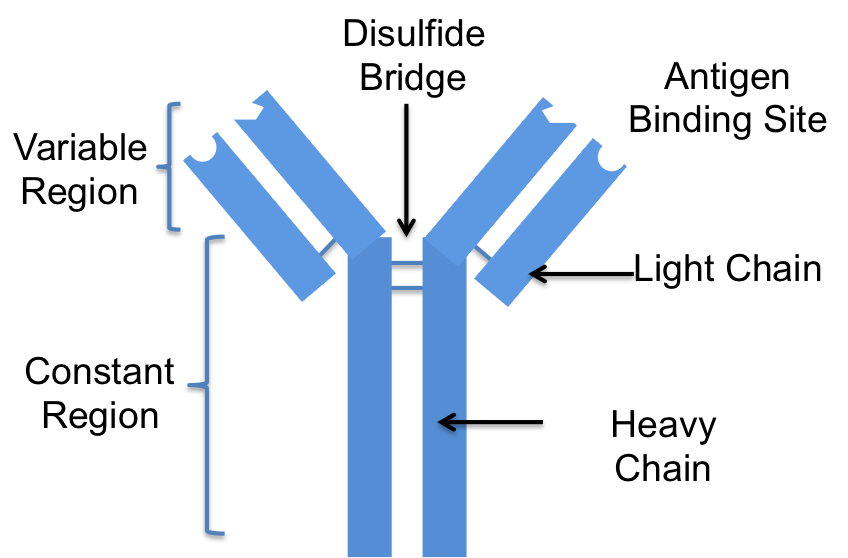
\includegraphics[width=0.7\textwidth]{antibody.png}
    \caption{Example figure inserted using a LaTeX Workshop snippet.}
    \label{fig:antibody}
\end{figure}

\subsection{Transducer Mechanisms}
The number of biological binding events indicates the concentration of the analyte in the sample. In order to convert the bio-recognition event into a measurable signal, a transducer mechanism is needed\cite{bhallaIntroductionBiosensors2016}. There are various types of transducer mechanisms that can be used in biosensors, including optical, piezoelectric and electrochemical transducers. This project will focus on biosensors where binding events change the electrical properties of the biosensor, specifically the complex impedance. Thus, electrochemical transducers are of interest. 

Electrochemical transducers can use various analysis techniques. In potentiometric analysis, the potential of an electrode is measured against a reference electrode at zero-current \cite{magarElectrochemicalImpedanceSpectroscopy2021}. Coulometry applies a constant potential (with regards to a reference electrode) onto an electrode surface to carry out exhaustive electrolysis of an analyte \cite{magarElectrochemicalImpedanceSpectroscopy2021}. Voltammetry involves subjecting the sample to a varying potential at the electrode's surface and measuring the resulting Faradaic current \cite{magarElectrochemicalImpedanceSpectroscopy2021}. Finally there is electrochemical impedance spectroscopy (EIS), which measures the complex impedance of an electrochemical system as a function of frequency \cite{magarElectrochemicalImpedanceSpectroscopy2021}. EIS is particularly suitable for biosensor applications where biological binding events alter the electrical properties of the electrode-electrolyte interface \cite{danielsLabelFreeImpedanceBiosensors2007}. This project will thus make use of EIS as the transduction mechanism.

\subsubsection{Electrochemical Impedance Spectroscopy}
This technique applies a small sinusoidal voltage signal to the biosensor and measures the resulting current response. The complex impedance is calculated as:
\begin{equation}
    Z(\omega) = \frac{V(\omega)}{I(\omega)} = Z'(\omega) + jZ''(\omega)
\end{equation}
where $Z'(\omega)$ is the real component representing resistive behaviour and $Z''(\omega)$ is the imaginary component representing capacitive or inductive behaviour.\cite{orazemTutorialElectrochemicalImpedance2020}

\subsubsection{Faradaic vs Non-Faradaic EIS Sensors}
EIS biosensors can be categorized into two main types based on their transduction mechanism: faradaic and non-faradaic sensors.\cite{dorledodefariaFaradaicNonfaradaicElectrochemical2019}

Faradaic sensors rely on electron transfer reactions at the electrode surface, typically requiring redox-active species in solution. These sensors detect changes in charge transfer resistance ($R_{ct}$) when biomolecule binding blocks electrode access or alters electron transfer kinetics. The equivalent circuit model for faradaic sensors is the Randles circuit, consisting of solution resistance ($R_s$) in series with the parallel combination of charge transfer resistance and double-layer capacitance ($C_{dl}$), plus Warburg impedance ($Z_w$) representing diffusion processes:
\begin{equation}
    Z = R_s + \frac{R_{ct}}{1 + j\omega R_{ct}C_{dl}} + Z_w
\end{equation}

Non-faradaic sensors operate without electron transfer reactions, functioning as capacitive sensors that detect changes in the electrical double layer capacitance. These sensors are particularly advantageous for biomarker detection as they require only simple electrolyte solutions and avoid complications associated with redox probes \cite{huangCapacitiveBiosensorsLabelfree2024}. The simplified equivalent circuit consists of solution resistance in series with interfacial capacitance:
\begin{equation}
    Z = R_s + \frac{1}{j\omega C_{interface}}
\end{equation}

Non-faradaic sensors are capacitive in nature, measuring changes in the dielectric properties at the electrode-electrolyte interface when biomolecules bind to immobilized antibodies. When antigen binding occurs, the capacitance decreases due to the displacement of water molecules and changes in the local dielectric constant according to:
\begin{equation}
    C = \frac{\varepsilon_0 \varepsilon_r A}{d}
\end{equation}
where $\varepsilon_0$ is the permittivity of free space, $\varepsilon_r$ is the relative permittivity of the medium, $A$ is the electrode area, and $d$ is the effective thickness of the dielectric layer.\cite{bergveldThirtyYearsBiosensor2003}
\todo{Discuss nyquist lower vs higher frequency and different effects at different frequencies}
\todo{Insert circuit models for faradaic and non-faradaic sensors}

% \subsubsection{Implementation for CA-19 Detection}
% The capacitive biosensors used in this project are designed to detect the CA-19 biomarker for pancreatic cancer screening. The frequency range for capacitive measurements typically spans from 1 Hz to 100 kHz, with the optimal frequency determined by the time constant $\tau = R_s C_{interface}$. At frequencies much higher than $1/\tau$, the impedance is dominated by solution resistance, while at frequencies much lower than $1/\tau$, the capacitive behaviour dominates the response.

\section{Signal Processing}
% The signal processing chain for EIS biosensors converts the electrochemical response into digital impedance measurements and ultimately biomarker concentrations. This process involves analogue front-end conditioning, digital signal processing, impedance calculation algorithms, and calibration models.\cite{katzElectrochemicalImpedanceSpectroscopy2021}

\subsection{Analogue Electronics}

\subsection{Digital Processing}

\subsection{Calculating Impedance}
% Complex impedance calculation requires extraction of magnitude and phase from voltage and current measurements. The impedance at frequency $\omega$ is calculated as:
% \begin{equation}
%     Z(\omega) = \frac{V(\omega)}{I(\omega)} = |Z|e^{j\phi} = Z' + jZ''
% \end{equation}
% where $Z'$ and $Z''$ are the real and imaginary components respectively.\cite{orazem2017electrochemical}

% Lock-in amplifier techniques provide high accuracy through synchronous detection. Digital implementation multiplies the input signal with sine and cosine reference waveforms, followed by low-pass filtering to extract DC components proportional to signal amplitude and phase.\cite{zuhriLockInAmplifier2022}

% Frequency sweep optimization employs logarithmic spacing with 10 points per decade across the measurement range. Descending frequency order (high to low) minimizes polarization effects and improves measurement accuracy for electrochemical systems.\cite{gamryBasicsElectrochemicalImpedance2024}

\subsection{Extrapolating from Impedance to Concentration}
% The conversion from impedance measurements to biomarker concentration requires equivalent circuit modeling and calibration. For capacitive biosensors, the simplified equivalent circuit consists of solution resistance $R_s$ in series with interfacial capacitance $C_{interface}$:
% \begin{equation}
%     Z = R_s + \frac{1}{j\omega C_{interface}}
% \end{equation}

% Biomarker binding alters the interfacial capacitance according to:
% \begin{equation}
%     C = \frac{\varepsilon_0 \varepsilon_r A}{d}
% \end{equation}
% where antigen binding increases the effective dielectric thickness $d$ and changes the local permittivity $\varepsilon_r$.\cite{songCapacitiveBiosensorsLabel2023}

% Calibration models relate impedance changes to analyte concentration. The Langmuir adsorption model describes the binding equilibrium:
% \begin{equation}
%     \theta = \frac{K_L C}{1 + K_L C}
% \end{equation}
% where $\theta$ is the fractional surface coverage, $K_L$ is the binding constant, and $C$ is the analyte concentration.\cite{langmuirAdsorptionModel2024}

% Non-linear least squares fitting, typically using the Levenberg-Marquardt algorithm, extracts equivalent circuit parameters from experimental impedance spectra.\cite{levenbergMarquardtAlgorithm2024} For CA-19 biosensors, detection limits of 0.1 U/mL are achievable with proper calibration and signal processing.\cite{kimCapacitiveBiosensorEarly2024}

\section{Interface}
\subsection{ESP32}
% \subsection{WebBLE}

\section{Related Works}

\label{chap:literature_review}